\chapter{Análisis de resultados}

%\begin{center}
%	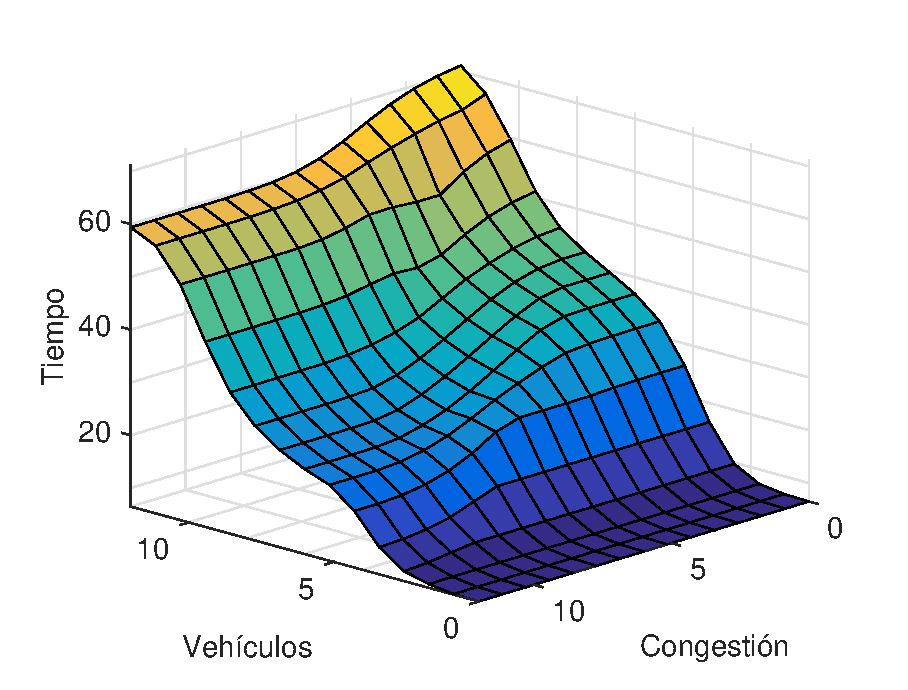
\includegraphics[width=11cm]{Surfaces/surface_d.eps}
%	\captionof{figure}{Superficie de control del sistema de inferencia}
%	\label{fig:surfaceControl}
%\end{center}

\section{Comparativa de las superficies de control}
Las siguientes figuras son las curvas de control generadas por cada una de las configuraciones probadas en la sección \ref{section:desarrolloFIS}, cada una de las curvas representa, mediante una gráfica de 3 dimensiones (una superficie), los valores de salida obtenidos por las distintas configuraciones.

\begin{figure}[H]
	\centering
	\subfigure[Superficie A]{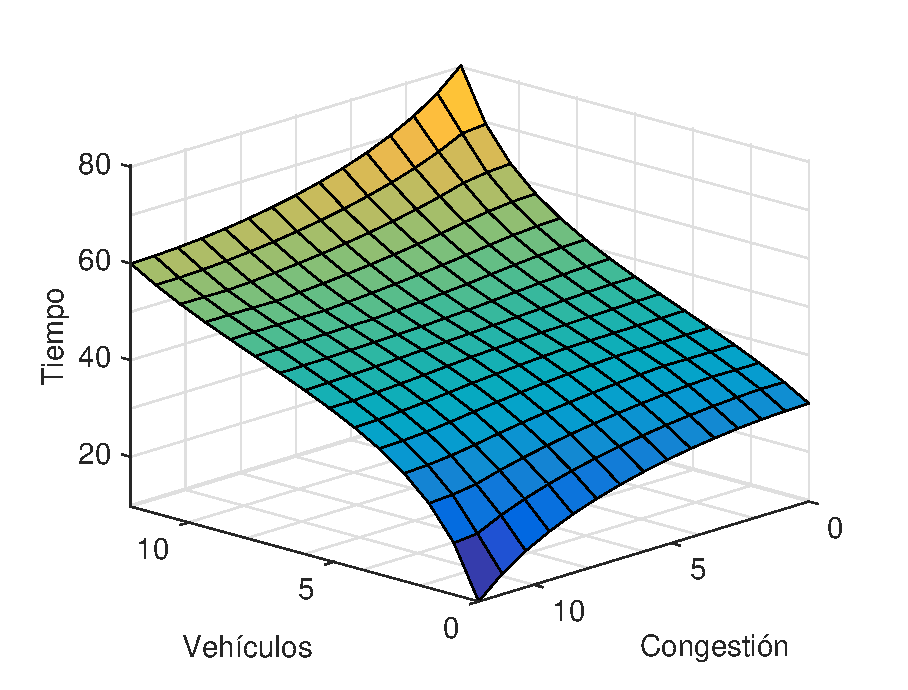
\includegraphics[width=8cm]{Surfaces/surface_a.eps}}
	\subfigure[Superficie B]{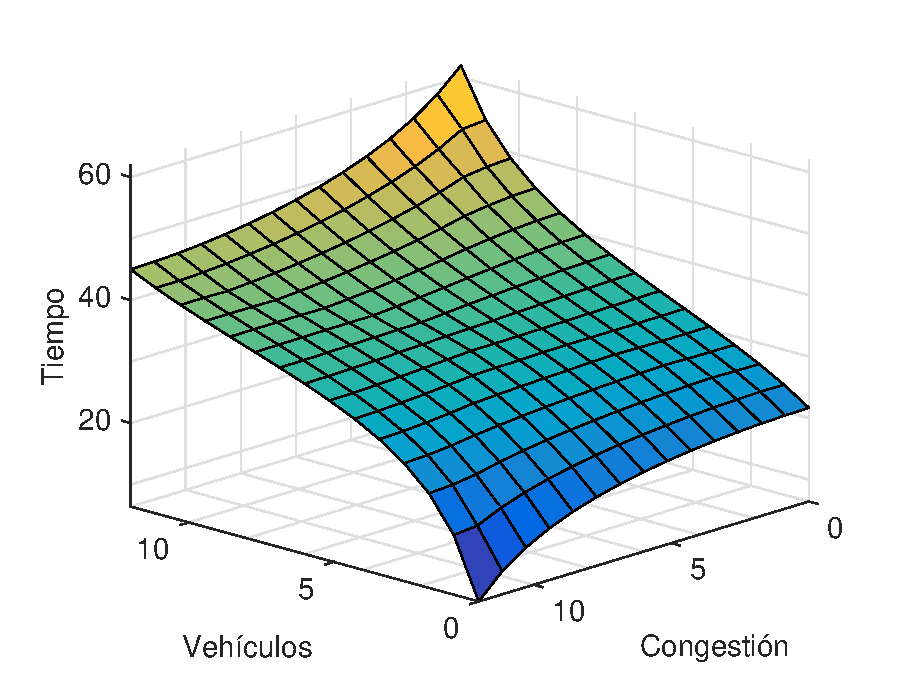
\includegraphics[width=8cm]{Surfaces/surface_b.eps}}
	\subfigure[Superficie C]{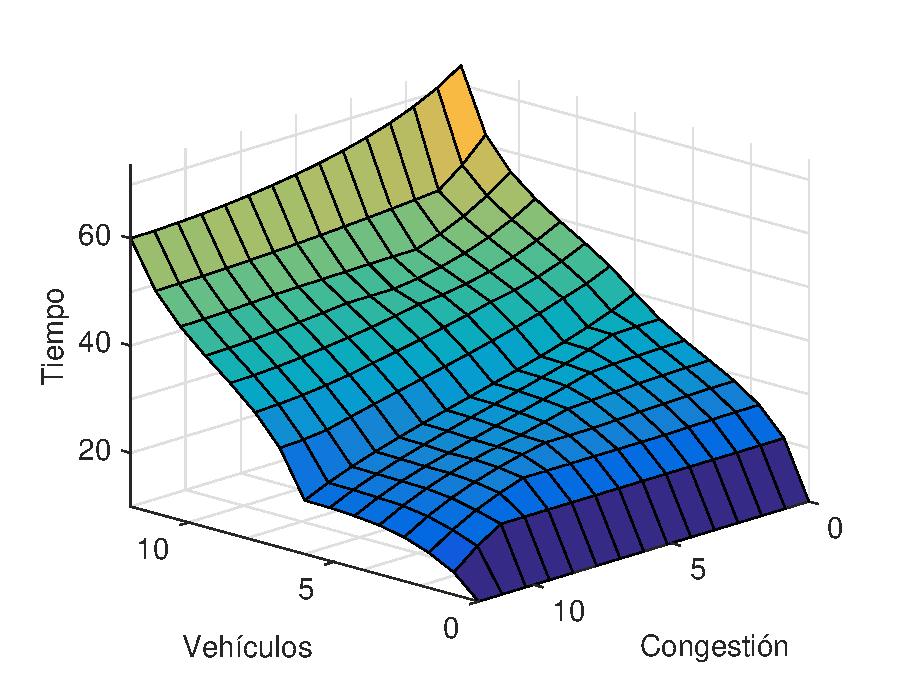
\includegraphics[width=8cm]{Surfaces/surface_c.eps}}
	\subfigure[Superficie D]{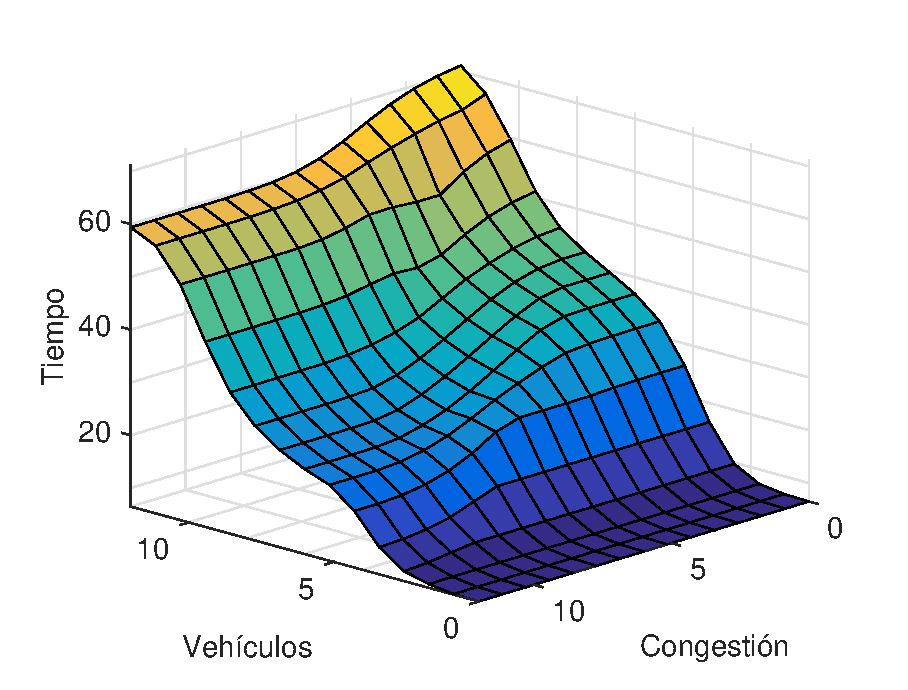
\includegraphics[width=8cm]{Surfaces/surface_d.eps}}
	\caption{Superficies de control}
\end{figure}

Las superficies mostradas arriba permiten ver el cambio gradual de las asignaciones de tiempo, de igual manera permiten apreciar la suavidad de la transición de los valores, además de que facilitan tener una perspectiva general de los valores de salida del sistema de inferencia.

Al analizar las gráficas se aprecia como las superficies A y B se ven afectadas de manera casi lineal por las variables de entrada. La diferencia más evidente es su rango de valores, pues la configuración A arroja valores de hasta 80s mientras que la B apenas rebasa los 60s.

En la superficie C se observa que existe un área donde la transición se vuelve un poco brusca e incluso toma una pendiente negativa. Este tipo de situaciones es más fácil observarlas cuando se recurre a una gráfica.

La superficie D, por otro lado, muestra una transición más limpia. También se observa como los valores de salida para congestiones altas se mantienen entre los 60s y 70s, mientras que para congestiones bajas se mantienen cerca a un mínimo de 10s.
Para valores de congestión entre 5 y 10, se observa como, con los mismos valores para la variable vehículos, aumenta hasta alcanzar un máximo que se mantiene en los 60s.

\section{Análisis de los repartos de tiempo}
Después de haber desarrollado y configurado la técnica seleccionada, ahora, en este capítulo se analizará el desempeño del algoritmo. Como se mencionó anteriormente, el algoritmo puede ser configurado para controlar intersecciones de diferente número de avenidas, carriles y avenidas. Con el fin de evaluar el desempeño del algoritmo frente a diferentes escenarios, se realizaron pruebas para los siguientes tipos de intersecciones que resultan ser las más comunes. 

{\setlength{\baselineskip}{0.5\baselineskip}
\begin{itemize}
	\item A: Intersecciones de 2 avenidas con 2 fases,
	\item B: Intersecciones de 4 avenidas con 2 fases y,
	\item C: Intersecciones de 4 avenidas con 4 fases.
\end{itemize}}

\textbf{Intersección A: 2 avenidas con 2 fases} Se entiende un cruce de dos calles de un solo sentido, donde el semáforo se encarga de ceder el paso de una sola de ellas en cada una de las fases (2 fases) tal y como se ve en la figura siguiente.
\begin{figure}[H]
	\centering
	\subfigure[Fase 1]{
	\begin{tikzpicture}[>=Triangle,scale=0.4]
		\clip (-4.5,4.5) rectangle (4.5,-4.5);	
		%calle eje x
		\fill[gray!50!white] (-4.5,1.5) rectangle (4.5,-1.5);
		%calle eje y
		\fill[gray!50!white] (-1.5,-4.5) rectangle (1.5,4.5);
		%semaforo
		\fill[black,scale=0.5] (3.35,1) rectangle (4,-1);
		\fill[black!30!red, scale=0.5] (3.65,0.65) circle(0.30);
		\fill[black!10!yellow, scale=0.5] (3.65,0) circle(0.30);
		\fill[black!60!green, scale=0.5] (3.65,-0.65) circle(0.30);
		%sentidos de las calles
		\draw[line width=0.6mm,->] (-4.5,0) -- (1.5,0);
		\draw [line width=0.6mm,->](-1.5,0) .. controls (0,0) and (0,0) .. (0,-3);
	\end{tikzpicture}
	}
	\subfigure[Fase 2]{
	
	\begin{tikzpicture}[>=Triangle,scale=0.4, rotate = 270]
		\clip (-4.5,4.5) rectangle (4.5,-4.5);
		%calle eje x
		\fill[gray!50!white] (-4.5,1.5) rectangle (4.5,-1.5);
		%calle eje y
		\fill[gray!50!white] (-1.5,-4.5) rectangle (1.5,4.5);
		%semaforo
		\fill[black,scale=0.5] (3.35,1) rectangle (4,-1);
		\fill[black!30!red, scale=0.5] (3.65,0.65) circle(0.30);
		\fill[black!10!yellow, scale=0.5] (3.65,0) circle(0.30);
		\fill[black!60!green, scale=0.5] (3.65,-0.65) circle(0.30);		
		%sentidos de las calles
		\draw[line width=0.6mm,->] (-4.5,0) -- (1.5,0);
		\draw [line width=0.6mm,->](-1.5,0) .. controls (0,0) and (0,0) .. (0,3);	
	\end{tikzpicture}
	}
	\caption{Intersección de 2 avenidas y 2 fases}
\end{figure}

\textbf{Intersección B: 4 avenidas con 2 fases.}
Se entiende un cruce de dos calles con doble sentido, donde el semáforo se encarga de ceder el paso a dos de ellas a la vez en cada fase, tal y como se ve en la figura siguiente. Normalmente se permite la vuelta a la izquierda con precaución.
\begin{figure}[H]
	\centering
	\subfigure[Fase 1]{
		\begin{tikzpicture}[>=Triangle,scale=0.4]
		\clip (-4.5,4.5) rectangle (4.5,-4.5);
		%calle eje x
		\fill[gray!50!white] (-4.5,1.5) rectangle (4.5,-1.5);
		%calle eje y
		\fill[gray!50!white] (-1.5,-4.5) rectangle (1.5,4.5);
		%semaforo
		\fill[black,scale=0.5] (-0.35,1) rectangle (0.35,-1);
		\fill[black!30!red, scale=0.5] (0,0.65) circle(0.30);
		\fill[black!10!yellow, scale=0.5] (0,0) circle(0.30);
		\fill[black!60!green, scale=0.5] (0,-0.65) circle(0.30);
		%division calles
		\draw [dashed,white,very thick] (-4.5,0) -- (-1.5,0);
		\draw [dashed,white,very thick] (6,1.5) -- (9,1.5);
		\draw [dashed,white,very thick] (0,4.5) -- (0,1.5);
		\draw [dashed,white,very thick] (0,-1.5) -- (0,-4.5);
		\draw [dashed,white,very thick] (1.5,0) -- (4.5,0);
		%sentidos de las calles
		\draw[line width=0.6mm,->] (-4.5,-0.75) -- (1.5,-0.75);
		\draw [line width=0.6mm,->](-1.5,-0.75) .. controls (-0.75,-0.75) and (-0.75,-0.75) .. (-0.75,-3);
		
		\draw[line width=0.6mm,->] (4.5,0.75) -- (-1.5,0.75);
		\draw [line width=0.6mm,->](1.5,0.75) .. controls (0.75,0.75) and (0.75,0.75) .. (0.75,3);
		\end{tikzpicture}
	}
	\subfigure[Fase 2]
	{
		\begin{tikzpicture}[>=Triangle, rotate= 90, scale=0.4]
		\clip (-4.5,4.5) rectangle (4.5,-4.5);
		%calle eje x
		\fill[gray!50!white] (-4.5,1.5) rectangle (4.5,-1.5);
		%calle eje y
		\fill[gray!50!white] (-1.5,-4.5) rectangle (1.5,4.5);
		%semaforo
		\fill[black,scale=0.5] (-0.35,1) rectangle (0.35,-1);
		\fill[black!30!red, scale=0.5] (0,0.65) circle(0.30);
		\fill[black!10!yellow, scale=0.5] (0,0) circle(0.30);
		\fill[black!60!green, scale=0.5] (0,-0.65) circle(0.30);
		%division calles
		\draw [dashed,white,very thick] (-4.5,0) -- (-1.5,0);
		\draw [dashed,white,very thick] (6,1.5) -- (9,1.5);
		\draw [dashed,white,very thick] (0,4.5) -- (0,1.5);
		\draw [dashed,white,very thick] (0,-1.5) -- (0,-4.5);
		\draw [dashed,white,very thick] (1.5,0) -- (4.5,0);
		%sentidos de las calles
		\draw[line width=0.6mm,->] (-4.5,-0.75) -- (1.5,-0.75);
		\draw [line width=0.6mm,->](-1.5,-0.75) .. controls (-0.75,-0.75) and (-0.75,-0.75) .. (-0.75,-3);
		
		\draw[line width=0.6mm,->] (4.5,0.75) -- (-1.5,0.75);
		\draw [line width=0.6mm,->](1.5,0.75) .. controls (0.75,0.75) and (0.75,0.75) .. (0.75,3);
		\end{tikzpicture}		
	}
	\caption{Intersección de 4 avenidas y 2 fases}
\end{figure}

\textbf{Intersección A: 4 avenidas con 2 fases.}
Se entiende un cruce de dos calles con doble sentido, donde el semáforo se encarga de ceder el paso a solo una de ellas en cada fase, tal y como se ve en la figura siguiente.
\begin{figure}[H]
	\centering
	\subfigure[Fase 1]
	{
		\begin{tikzpicture}[>=Triangle, scale=0.4]
		\clip (-4.5,4.5) rectangle (4.5,-4.5);
		%calle eje x
		\fill[gray!50!white] (-4.5,1.5) rectangle (4.5,-1.5);
		%calle eje y
		\fill[gray!50!white] (-1.5,-4.5) rectangle (1.5,4.5);
		%semaforo
		\fill[black,scale=0.5] (3.35,1) rectangle (4,-1);
		\fill[black!30!red, scale=0.5] (3.65,0.65) circle(0.30);
		\fill[black!10!yellow, scale=0.5] (3.65,0) circle(0.30);
		\fill[black!60!green, scale=0.5] (3.65,-0.65) circle(0.30);
		%division calles
		\draw [dashed,white,very thick] (-4.5,0) -- (-1.5,0);
		\draw [dashed,white,very thick] (6,1.5) -- (9,1.5);
		\draw [dashed,white,very thick] (0,4.5) -- (0,1.5);
		\draw [dashed,white,very thick] (0,-1.5) -- (0,-4.5);
		\draw [dashed,white,very thick] (2.5,0) -- (4.5,0);
		%sentidos de las calles
		\draw[line width=0.6mm,->] (-4.5,-0.75) -- (1.8,-0.75);
		\draw [line width=0.6mm,->](-1.5,-0.75) .. controls (-0.75,-0.75) and (-0.75,-0.75) .. (-0.75,-3);
		\draw [line width=0.6mm,->](-1.5,-0.75) .. controls (1,-0.75) and (1,-0.75) .. (1,3);
		\end{tikzpicture}		
	}
	\subfigure[Fase 2]
	{
		\begin{tikzpicture}[>=Triangle, scale=0.4, rotate=90]
		\clip (-4.5,4.5) rectangle (4.5,-4.5);
		%calle eje x
		\fill[gray!50!white] (-4.5,1.5) rectangle (4.5,-1.5);
		%calle eje y
		\fill[gray!50!white] (-1.5,-4.5) rectangle (1.5,4.5);
		%semaforo
		\fill[black,scale=0.5] (3.35,1) rectangle (4,-1);
		\fill[black!30!red, scale=0.5] (3.65,0.65) circle(0.30);
		\fill[black!10!yellow, scale=0.5] (3.65,0) circle(0.30);
		\fill[black!60!green, scale=0.5] (3.65,-0.65) circle(0.30);
		%division calles
		\draw [dashed,white,very thick] (-4.5,0) -- (-1.5,0);
		\draw [dashed,white,very thick] (6,1.5) -- (9,1.5);
		\draw [dashed,white,very thick] (0,4.5) -- (0,1.5);
		\draw [dashed,white,very thick] (0,-1.5) -- (0,-4.5);
		\draw [dashed,white,very thick] (2.5,0) -- (4.5,0);
		%sentidos de las calles
		\draw [line width=0.6mm,->] (-4.5,-0.75) -- (1.8,-0.75);
		\draw [line width=0.6mm,->](-1.5,-0.75) .. controls (-0.75,-0.75) and (-0.75,-0.75) .. (-0.75,-3);
		\draw [line width=0.6mm,->](-1.5,-0.75) .. controls (1,-0.75) and (1,-0.75) .. (1,3);
		\end{tikzpicture}
	}
	\subfigure[Fase 3]
	{
		\begin{tikzpicture}[>=Triangle, scale=0.4, rotate=180]
		\clip (-4.5,4.5) rectangle (4.5,-4.5);
		%calle eje x
		\fill[gray!50!white] (-4.5,1.5) rectangle (4.5,-1.5);
		%calle eje y
		\fill[gray!50!white] (-1.5,-4.5) rectangle (1.5,4.5);
		%semaforo
		\fill[black,scale=0.5] (3.35,1) rectangle (4,-1);
		\fill[black!30!red, scale=0.5] (3.65,0.65) circle(0.30);
		\fill[black!10!yellow, scale=0.5] (3.65,0) circle(0.30);
		\fill[black!60!green, scale=0.5] (3.65,-0.65) circle(0.30);
		%division calles
		\draw [dashed,white,very thick] (-4.5,0) -- (-1.5,0);
		\draw [dashed,white,very thick] (6,1.5) -- (9,1.5);
		\draw [dashed,white,very thick] (0,4.5) -- (0,1.5);
		\draw [dashed,white,very thick] (0,-1.5) -- (0,-4.5);
		\draw [dashed,white,very thick] (2.5,0) -- (4.5,0);
		%sentidos de las calles
		\draw [line width=0.6mm,->] (-4.5,-0.75) -- (1.8,-0.75);
		\draw [line width=0.6mm,->](-1.5,-0.75) .. controls (-0.75,-0.75) and (-0.75,-0.75) .. (-0.75,-3);
		\draw [line width=0.6mm,->](-1.5,-0.75) .. controls (1,-0.75) and (1,-0.75) .. (1,3);
		\end{tikzpicture}
	}
	\subfigure[Fase 4]
	{
		\begin{tikzpicture}[>=Triangle, scale=0.4, rotate=270]
		\clip (-4.5,4.5) rectangle (4.5,-4.5);
		%calle eje x
		\fill[gray!50!white] (-4.5,1.5) rectangle (4.5,-1.5);
		%calle eje y
		\fill[gray!50!white] (-1.5,-4.5) rectangle (1.5,4.5);
		%semaforo
		\fill[black,scale=0.5] (3.35,1) rectangle (4,-1);
		\fill[black!30!red, scale=0.5] (3.65,0.65) circle(0.30);
		\fill[black!10!yellow, scale=0.5] (3.65,0) circle(0.30);
		\fill[black!60!green, scale=0.5] (3.65,-0.65) circle(0.30);
		%division calles
		\draw [dashed,white,very thick] (-4.5,0) -- (-1.5,0);
		\draw [dashed,white,very thick] (6,1.5) -- (9,1.5);
		\draw [dashed,white,very thick] (0,4.5) -- (0,1.5);
		\draw [dashed,white,very thick] (0,-1.5) -- (0,-4.5);
		\draw [dashed,white,very thick] (2.5,0) -- (4.5,0);
		%sentidos de las calles
		\draw [line width=0.6mm,->] (-4.5,-0.75) -- (1.8,-0.75);
		\draw [line width=0.6mm,->](-1.5,-0.75) .. controls (-0.75,-0.75) and (-0.75,-0.75) .. (-0.75,-3);
		\draw [line width=0.6mm,->](-1.5,-0.75) .. controls (1,-0.75) and (1,-0.75) .. (1,3);
		\end{tikzpicture}
	}
	\caption{Intersección de 4 avenidas y 4 fases.}
\end{figure}



\textbf{Para cada una de las intersecciones} se suministra un conjunto de valores de prueba. Los valores inferidos por el algoritmo son presentados a manera de tablas en las siguientes secciones.





\newpage
\subsection{Intersección de 2 avenidas y 2 fases}
La siguiente tabla muestra los valores (aleatorios) de entrada suministrados para cada una de las 4 pruebas realizadas, cada uno de los valores representa la cantidad de autos por avenida. Además, se observa el número de carriles de cada avenida y las avenidas que intervienen en cada \emph{fase en verde}.

\begin{longtable}[c]{ccccc} \toprule
	\textbf{No} &\multicolumn{2}{c}{\textbf{Vehículos}} & \multicolumn{2}{c}{\textbf{Tiempos asignados}} \\[0.2cm]
	&  Avenida 1 & Avenida 2 & Fase 1 & Fase 2 \\[0cm]
	&{\scriptsize(1 carril)}&{\scriptsize (1 carril)} &{\scriptsize (av 1)} &{\scriptsize(av 2)} \\[0.1cm]\midrule
	1 & 1 & 8 & 8.58 &43.09\\
	3 & 4 & 7 & 22.29 & 35.74\\
	2 & 12 & 5 & 61.69 & 21.40\\
	4 & 12 & 10 & 59.39 & 48.29\\\bottomrule
	\caption{Valores de prueba para la intersección A}
\end{longtable}

Las siguientes gráficas representan los repartos de tiempo para cada conjunto de valores de prueba. A diferencia de una asignación estática, aquí se observa como los tiempos varían en función de la cantidad de vehículos.

\begin{figure}[H]
	\centering
	\subfigure[Prueba No. 1]{\begin{tikzpicture}[scale=0.4]\pie[style=drop shadow, sum=auto, text=legend, after number={s}, cloud]{8.6/{Fase 1}, 43.1/{Fase 2} } \end{tikzpicture} }
	\subfigure[Prueba No. 2]{\begin{tikzpicture}[scale=0.4]\pie[style=drop shadow, sum=auto, text=legend, after number={s}, cloud]{22.3/{Fase 1}, 35.7/{Fase 2} } \end{tikzpicture} }\\
	\subfigure[Prueba No. 3]{\begin{tikzpicture}[scale=0.4]\pie[style=drop shadow, sum=auto, text=legend, after number=s, cloud]{61.7/{Fase 1}, 21.4/{Fase 2} } \end{tikzpicture} }
	\subfigure[Prueba No. 4]{\begin{tikzpicture}[scale=0.4]\pie[style=drop shadow, sum=auto, text=legend, after number=s, cloud]{59.4/{Fase 1}, 48.3/{Fase 2} } \end{tikzpicture} }
	\caption{Repartos de tiempo de la intersección A}
\end{figure}





\newpage
\subsection{Intersección de 4 avenidas y 2 fases}
Al igual que en la sección anterior, se observa los valores de prueba suministrados y los tiempos inferidos por el sistema de inferencia, también se observa el número de carriles de cada avenida y las avenidas que intervienen en cada \emph{fase en verde}.
\begin{longtable}[c]{ccccccc} \toprule
	\textbf{No} &\multicolumn{4}{c}{\textbf{Vehículos}} & \multicolumn{2}{c}{\textbf{Tiempos asignados}} \\[0.2cm]
	&  Avenida 1 & Avenida 2 &  Avenida 3 & Avenida 4 & Fase 1 & Fase 2 \\[0cm]
	&{\scriptsize(2 carriles)}&{\scriptsize (1 carril)} &{\scriptsize (2 carriles)} & {\scriptsize (1 carril)} &{\scriptsize (avs 1 y 3)} &{\scriptsize(avs 1 y 4)} \\[0.1cm]\midrule
	1 & 1 & 8 & 8 & 10 & 9.45 &45.68\\
	3 & 2 & 4 & 8 & 12 & 9.45 & 42.04\\
	2 & 20 & 10 & 12 & 5 & 31.53 & 27.09\\
	4 & 30 & 12 & 7 & 5 & 37.76& 30.86 \\\bottomrule
	\caption{Valores de prueba para la intersección B}
\end{longtable}

Las siguientes gráficas representan los repartos de tiempo para cada conjunto de valores de prueba.
\begin{figure}[H]
	\centering
	\subfigure[Prueba No. 1]{\begin{tikzpicture}[scale=0.4]\pie[style=drop shadow, sum=auto, text=legend, after number={s}, cloud]{9.45/{Fase 1}, 45.68/{Fase 2} } \end{tikzpicture} }
	\subfigure[Prueba No. 2]{\begin{tikzpicture}[scale=0.4]\pie[style=drop shadow, sum=auto, text=legend, after number={s}, cloud]{9.45/{Fase 1}, 42.04/{Fase 2} } \end{tikzpicture} }\\
	\subfigure[Prueba No. 3]{\begin{tikzpicture}[scale=0.4]\pie[style=drop shadow, sum=auto, text=legend, after number=s, cloud]{31.53/{Fase 1}, 27.09/{Fase 2} } \end{tikzpicture} }
	\subfigure[Prueba No. 4]{\begin{tikzpicture}[scale=0.4]\pie[style=drop shadow, sum=auto, text=legend, after number=s, cloud]{37.76/{Fase 1}, 30.86/{Fase 2} } \end{tikzpicture} }
	\caption{Repartos de tiempo de la intersección B}
\end{figure}




\newpage
\subsection{Intersección de 4 avenidas y 4 fases}
Al igual que en las secciones anteriores, se observa los valores de prueba suministrados y los tiempos inferidos, también se observa el número de carriles de cada avenida y las avenidas que intervienen en cada \emph{fase en verde}.

\begin{longtable}[c]{ccccccccc} \toprule
	\textbf{No} & \multicolumn{4}{c}{\textbf{Vehículos}} & \multicolumn{4}{c}{\textbf{Tiempos asignados}} \\[0.2cm]
	
	&  Avenida 1 & Avenida 2 &  Avenida 3 & Avenida 4 & Fase 1 & Fase 2 & Fase 3 & Fase 4\\[0cm]
	
	&{\scriptsize(3 carriles)}&{\scriptsize (2 carriles)}
	&{\scriptsize(2 carriles)}&{\scriptsize (1 carril)}
	&{\scriptsize (av 1)} &{\scriptsize(av 2)}
	&{\scriptsize (av 3)} &{\scriptsize(av 2)} \\[0.1cm]\midrule
	
	1 & 2 	& 8		& 8 	& 10 	& 08.44 & 22.43 & 22.43 & 52.65 \\
	3 & 2 	& 4 	& 8 	& 12 	& 08.44 & 09.45 & 22.43 & 70.07 \\
	2 & 20 	& 10 	& 12 	& 5 	& 31.42 & 28.09 & 31.52 & 28.09\\
	4 & 30 	& 12	& 7 	& 5 	& 49.76 & 26.63 & 13.28 & 25.59 \\\bottomrule
	\caption{Valores de prueba para la intersección C}
\end{longtable}

El reparto de tiempos es el siguiente:
\begin{figure}[H]
	\centering
	\subfigure[Prueba No. 1]{\begin{tikzpicture}[scale=0.5]\pie[style=drop shadow, sum=auto, text=legend, after number={s}, cloud]
		{8.4/{Fase 1}, 22.4/{Fase 2}, 22.4/{Fase 3}, 52.7/{Fase 4} } \end{tikzpicture} }
	\subfigure[Prueba No. 2]{\begin{tikzpicture}[scale=0.5]\pie[style=drop shadow, sum=auto, text=legend, after number={s}, cloud]
		{8.4/{Fase 1}, 9.5/{Fase 2}, 22.4/{Fase 3}, 70.1/{Fase 4} } \end{tikzpicture} }\\
	\subfigure[Prueba No. 3]{\begin{tikzpicture}[scale=0.5]\pie[style=drop shadow, sum=auto, text=legend, after number={s}, cloud]
		{31.4/{Fase 1}, 28.1/{Fase 2}, 31.5/{Fase 3}, 28.1/{Fase 4} } \end{tikzpicture} }
	\subfigure[Prueba No. 4]{\begin{tikzpicture}[scale=0.5]\pie[style=drop shadow, sum=auto, text=legend, after number={s}, cloud]
		{49.8/{Fase 1}, 26.6/{Fase 2}, 13.3/{Fase 3}, 25.6/{Fase 4} } \end{tikzpicture} }
	\caption{Repartos de tiempo de la intersección C}
\end{figure}
